\documentclass[11pt]{IEEEphot}

\usepackage{setspace}
\usepackage{tikz}
\usepackage{amsmath, amssymb}
\usepackage{slashbox}
\usepackage{algorithm,algpseudocode}
\usepackage{mathrsfs}
\usepackage{setspace}
\usepackage{caption}
\usepackage{pgfplots}


\classnumber{CS 5300}

\newtheorem{theorem}{Theorem}
\newtheorem{lemma}{Lemma}

\doublespacing
\begin{document}
	
	\title{An Analysis\\ of \\ Branch-and-Bound}
	
	\author{~Rick Ramirez \\ Ruben Bramasco}
	
	\affil{California State Polytechnic University, Pomona}
	\maketitle
	\markboth{Fall 2021}{Advanced Algorithm Design and Analysis}
	\vspace{-2cm}
	\begin{center}
    	
\includegraphics[width=5cm]{images/primary-logo-inside-stacked}\\
    \end{center}
	\vspace{0.25cm}

	\begin{abstract}
		\doublespacing\small
		The Branch-and-Bound paradigm is a widely used framework for solving combinatorial optimization problems.
		Here we describe the general algorithm and show how it can be broken into various sub-routines. 
		For each sub-routine, we describe when it is appropriate to use it and analyze it's effect on performance.
		We follow this with two applications involving an integer constraint problem and the traveling salesman problem. 
		Finally, we close with a discussion of recent improvements of the branch-and-bound framework in the wake of quantum computation and describe how a quantum algorithm could produce a quadratic acceleration of the classical time complexity.
	\end{abstract}

	\begin{IEEEkeywords}
		Branch-and-Bound, Pruning rules, Branching strategy, Ising model, Quantum walk
	\end{IEEEkeywords}

	%! Author = rickr
%! Date = 11/17/2021

\section{Introduction}

	
	%! Author = rickr
%! Date = 11/17/2021
\newpage
\section{Basic Idea Behind BnB}
	
		%! Author = rickr
%! Date = 11/27/2021
\subsection{Search Strategies}
	Searching strategies used in branch-and-bound algorithms determine the order in which sub-problems are explored. The three most common techniques are, depth-first search, breadth-first search, and best-first search. 
	Each technique is well suited for a particular scenario and the choice of search strategy for a particular problem could have a significant impact on performance and/or memory requirements.
	\begin{figure}[h]
		\begin{center}
			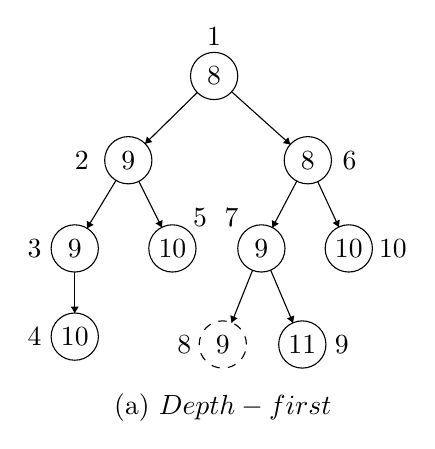
\begin{tikzpicture}[scale=0.1]
				\tikzstyle{every node}+=[inner sep=0pt]
				\draw [black] (34.8,-8) circle (3);
				\draw (34.8,-8) node {$8$};
				\draw (34.8,-3) node {$1$};
				\draw [black] (23.9,-18.7) circle (3);
				\draw (23.9,-18.7) node {$9$};
				\draw (18,-18.7) node {$2$};
				\draw [black] (46.7,-18.7) circle (3);
				\draw (46.7,-18.7) node {$8$};
				\draw (52,-18.7) node {$6$};
				\draw [black] (17.1,-29.9) circle (3);
				\draw (17.1,-29.9) node {$9$};
				\draw (12,-29.9) node {$3$};
				\draw [black] (29.5,-29.9) circle (3);
				\draw (29.5,-29.9) node {$10$};
				\draw (33,-26) node {$5$};
				\draw [black] (17.1,-41.1) circle (3);
				\draw (17.1,-41.1) node {$10$};
				\draw (12,-41.1) node {$4$};
				\draw [black] (40.8,-29.9) circle (3);
				\draw (40.8,-29.9) node {$9$};
				\draw (37,-26) node {$7$};
				\draw [black] (51.9,-29.9) circle (3);
				\draw (51.9,-29.9) node {$10$};
				\draw (57.5,-29.9) node {$10$};
				\draw [dashed] (35.9,-42.1) circle (3);
				\draw (35.9,-42.1) node {$9$};
				\draw (31,-42.1) node {$8$};
				\draw [black] (46,-42.1) circle (3);
				\draw (46,-42.1) node {$11$};
				\draw (51,-42.1) node {$9$};
				\draw [black] (32.66,-10.1) -- (26.04,-16.6);
				\fill [black] (26.04,-16.6) -- (26.96,-16.39) -- (26.26,-15.68);
				\draw [black] (37.03,-10.01) -- (44.47,-16.69);
				\fill [black] (44.47,-16.69) -- (44.21,-15.79) -- (43.54,-16.53);
				\draw [black] (22.34,-21.26) -- (18.66,-27.34);
				\fill [black] (18.66,-27.34) -- (19.5,-26.91) -- (18.64,-26.39);
				\draw [black] (25.24,-21.38) -- (28.16,-27.22);
				\fill [black] (28.16,-27.22) -- (28.25,-26.28) -- (27.35,-26.72);
				\draw [black] (17.1,-32.9) -- (17.1,-38.1);
				\fill [black] (17.1,-38.1) -- (17.6,-37.3) -- (16.6,-37.3);
				\draw [black] (39.68,-32.68) -- (37.02,-39.32);
				\fill [black] (37.02,-39.32) -- (37.78,-38.76) -- (36.85,-38.39);
				\draw [black] (41.98,-32.66) -- (44.82,-39.34);
				\fill [black] (44.82,-39.34) -- (44.97,-38.41) -- (44.05,-38.8);
				\draw [black] (45.3,-21.35) -- (42.2,-27.25);
				\fill [black] (42.2,-27.25) -- (43.01,-26.77) -- (42.13,-26.3);
				\draw [black] (47.96,-21.42) -- (50.64,-27.18);
				\fill [black] (50.64,-27.18) -- (50.75,-26.24) -- (49.85,-26.66);
				\draw (35.9,-50.1) node {$\text{(a) }Depth-first$};
			\end{tikzpicture}\qquad
			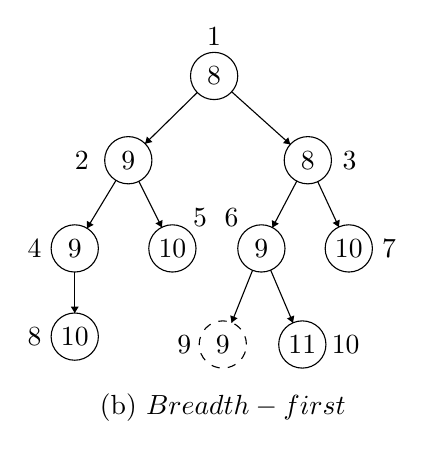
\begin{tikzpicture}[scale=0.1]
				\tikzstyle{every node}+=[inner sep=0pt]
				\draw [black] (34.8,-8) circle (3);
				\draw (34.8,-8) node {$8$};
				\draw (34.8,-3) node {$1$};
				\draw [black] (23.9,-18.7) circle (3);
				\draw (23.9,-18.7) node {$9$};
				\draw (18,-18.7) node {$2$};
				\draw [black] (46.7,-18.7) circle (3);
				\draw (46.7,-18.7) node {$8$};
				\draw (52,-18.7) node {$3$};
				\draw [black] (17.1,-29.9) circle (3);
				\draw (17.1,-29.9) node {$9$};
				\draw (12,-29.9) node {$4$};
				\draw [black] (29.5,-29.9) circle (3);
				\draw (29.5,-29.9) node {$10$};
				\draw (33,-26) node {$5$};
				\draw [black] (17.1,-41.1) circle (3);
				\draw (17.1,-41.1) node {$10$};
				\draw (12,-41.1) node {$8$};
				\draw [black] (40.8,-29.9) circle (3);
				\draw (40.8,-29.9) node {$9$};
				\draw (37,-26) node {$6$};
				\draw [black] (51.9,-29.9) circle (3);
				\draw (51.9,-29.9) node {$10$};
				\draw (57,-29.9) node {$7$};
				\draw [dashed] (35.9,-42.1) circle (3);
				\draw (35.9,-42.1) node {$9$};
				\draw (31,-42.1) node {$9$};
				\draw [black] (46,-42.1) circle (3);
				\draw (46,-42.1) node {$11$};
				\draw (51.5,-42.1) node {$10$};
				\draw [black] (32.66,-10.1) -- (26.04,-16.6);
				\fill [black] (26.04,-16.6) -- (26.96,-16.39) -- (26.26,-15.68);
				\draw [black] (37.03,-10.01) -- (44.47,-16.69);
				\fill [black] (44.47,-16.69) -- (44.21,-15.79) -- (43.54,-16.53);
				\draw [black] (22.34,-21.26) -- (18.66,-27.34);
				\fill [black] (18.66,-27.34) -- (19.5,-26.91) -- (18.64,-26.39);
				\draw [black] (25.24,-21.38) -- (28.16,-27.22);
				\fill [black] (28.16,-27.22) -- (28.25,-26.28) -- (27.35,-26.72);
				\draw [black] (17.1,-32.9) -- (17.1,-38.1);
				\fill [black] (17.1,-38.1) -- (17.6,-37.3) -- (16.6,-37.3);
				\draw [black] (39.68,-32.68) -- (37.02,-39.32);
				\fill [black] (37.02,-39.32) -- (37.78,-38.76) -- (36.85,-38.39);
				\draw [black] (41.98,-32.66) -- (44.82,-39.34);
				\fill [black] (44.82,-39.34) -- (44.97,-38.41) -- (44.05,-38.8);
				\draw [black] (45.3,-21.35) -- (42.2,-27.25);
				\fill [black] (42.2,-27.25) -- (43.01,-26.77) -- (42.13,-26.3);
				\draw [black] (47.96,-21.42) -- (50.64,-27.18);
				\fill [black] (50.64,-27.18) -- (50.75,-26.24) -- (49.85,-26.66);
				\draw (35.9,-50.1) node {$\text{(b) }Breadth-first$};
			\end{tikzpicture}\qquad
			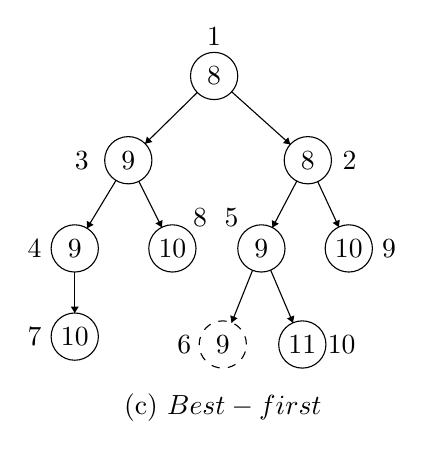
\begin{tikzpicture}[scale=0.1]
				\tikzstyle{every node}+=[inner sep=0pt]
				\draw [black] (34.8,-8) circle (3);
				\draw (34.8,-8) node {$8$};
				\draw (34.8,-3) node {$1$};
				\draw [black] (23.9,-18.7) circle (3);
				\draw (23.9,-18.7) node {$9$};
				\draw (18,-18.7) node {$3$};
				\draw [black] (46.7,-18.7) circle (3);
				\draw (46.7,-18.7) node {$8$};
				\draw (52,-18.7) node {$2$};
				\draw [black] (17.1,-29.9) circle (3);
				\draw (17.1,-29.9) node {$9$};
				\draw (12,-29.9) node {$4$};
				\draw [black] (29.5,-29.9) circle (3);
				\draw (29.5,-29.9) node {$10$};
				\draw (33,-26) node {$8$};
				\draw [black] (17.1,-41.1) circle (3);
				\draw (17.1,-41.1) node {$10$};
				\draw (12,-41.1) node {$7$};
				\draw [black] (40.8,-29.9) circle (3);
				\draw (40.8,-29.9) node {$9$};
				\draw (37,-26) node {$5$};
				\draw [black] (51.9,-29.9) circle (3);
				\draw (51.9,-29.9) node {$10$};
				\draw (57,-29.9) node {$9$};
				\draw [dashed] (35.9,-42.1) circle (3);
				\draw (35.9,-42.1) node {$9$};
				\draw (31,-42.1) node {$6$};
				\draw [black] (46,-42.1) circle (3);
				\draw (46,-42.1) node {$11$};
				\draw (51,-42.1) node {$10$};
				\draw [black] (32.66,-10.1) -- (26.04,-16.6);
				\fill [black] (26.04,-16.6) -- (26.96,-16.39) -- (26.26,-15.68);
				\draw [black] (37.03,-10.01) -- (44.47,-16.69);
				\fill [black] (44.47,-16.69) -- (44.21,-15.79) -- (43.54,-16.53);
				\draw [black] (22.34,-21.26) -- (18.66,-27.34);
				\fill [black] (18.66,-27.34) -- (19.5,-26.91) -- (18.64,-26.39);
				\draw [black] (25.24,-21.38) -- (28.16,-27.22);
				\fill [black] (28.16,-27.22) -- (28.25,-26.28) -- (27.35,-26.72);
				\draw [black] (17.1,-32.9) -- (17.1,-38.1);
				\fill [black] (17.1,-38.1) -- (17.6,-37.3) -- (16.6,-37.3);
				\draw [black] (39.68,-32.68) -- (37.02,-39.32);
				\fill [black] (37.02,-39.32) -- (37.78,-38.76) -- (36.85,-38.39);
				\draw [black] (41.98,-32.66) -- (44.82,-39.34);
				\fill [black] (44.82,-39.34) -- (44.97,-38.41) -- (44.05,-38.8);
				\draw [black] (45.3,-21.35) -- (42.2,-27.25);
				\fill [black] (42.2,-27.25) -- (43.01,-26.77) -- (42.13,-26.3);
				\draw [black] (47.96,-21.42) -- (50.64,-27.18);
				\fill [black] (50.64,-27.18) -- (50.75,-26.24) -- (49.85,-26.66);
				\draw (35.9,-50.1) node {$\text{(c) } Best-first$};
			\end{tikzpicture}\qquad
		\end{center}
		\caption{\doublespacing Sub-tree traversals for different searching techniques. The numbers on the side of each node correspond to the lower-bound at that step and the dotted node represents the optimal solution \cite{morrison2016branch}.}
		\label{fig:searchTechniques}
	\end{figure}
		\subsubsection{Depth-First}
			The depth-first search strategy follows a last-in, first-out order and is implemented by maintaining a list of unexplored nodes in a stack as shown in Figure \ref{fig:searchTechniques} (a). 
			The routine removes the top element from the stack to explore for the next sub-problem and the children generated are inserted on the top of the stack. The potential memory requirements needed to maintain a list of children nodes can become a problem, however we remedy this by maintaining a path of indices from the root to the current node instead of the entire list of unexplored sub-problems.
			When the current sub-problem is complete, the algorithm selects the next unexplored node for exploration and if one does not exist, the algorithm backtracks to the nearest ancestor node. 
			The biggest issue with this technique is that it is blind to the structure of the problem and makes no use of the lower bounds encountered during a traversal. 
			This can cause the algorithm to spend large amounts of time exploring unpromising regions, especially when the search space is unbalanced. 
			This results in a running time of $\Theta (V+E)$ \cite{cormen2009introduction}, however DFS yields valuable information about the structure of a graph.
		\subsubsection{Breadth-First}
			The breadth-first search strategy, shown in Figure \ref{fig:searchTechniques} (b), explores nodes based on a first-in, first-out order and is implemented by maintaining a queue data structure. 
			This results in the algorithm exploring all nodes at the same level before moving on to deeper portions of the tree. 
			The advantage of this technique is that if the optimal solution is close to the root, or the tree is unbalanced, breadth-first search will find the solution faster than depth-first. 
			However, if the solution occurs at lower depths, breadth-first can require large amounts of memory because it does not take advantage of any pruning rules. 
			The BFS technique runs on a running time of $O(V+E)$ \cite{cormen2009introduction} and is linear to the size of an adjacency list representation of the graph.
		\subsubsection{Best-First}
			The best-first search strategy is often used when memory considerations are of no concern. This technique stores the entire unexplored search space and applies a heuristic function to every unexplored node and selects the node that returns the minimum value. 
			We say that the heuristic function is admissible if it never overestimates the best solution and is often referred to as the $A^*$  method. The technique is implemented as a heap data structure and the order of a traversal can be seen in Figure \ref{fig:searchTechniques} (c). 
			The complexity of $A^*$ depends on the heuristic used.
			In an unbounded search space, the worst case running time can reach $O(b^d)$ \cite{russell2010artificial} where $d$ is the shortest path to a solution and $b$ is the branching factor. 

		%! Author = rickr
%! Date = 11/17/2021

\subsection{Pruning Rules}
	The pruning rules of Algorithm \ref{alg: pseudocode} determine whether or not $S$ can be fathomed.
	While the use of a heuristic allows us to approximate the utility of a state without performing a complete search, pruning rules allow us to neglect portions of the tree without affecting the final choice. 
	Many of the pruning techniques are developed in the context of Artificial Intelligence, however the basic function holds across all applications involving combinatorial optimization. 
	\subsubsection{Lower-Bound}
		Producing a lower bound on the objective function at each node is the most common way to prune a search space \cite{morrison2016branch}. 
		The lower bound then used to prune sub-problems who's lower bound is no better than the incumbent solution. 
		The value of the lower bound is calculated by relaxing aspects of the problem, and as such, some lower bound calculations may be easier to determine than others. 
		The general technique is to attempt pruning with a lower bound that is easy to calculate before moving on to more complex (but possibly tighter) lower bounds. 
	\subsubsection{Alpha-Beta Pruning}
		Alpha-beta pruning is often used in areas of artificial intelligence that employ a MinMax decision rule for minimizing the possible loss of a worst case scenario. 
		The idea is to maximize the minimum gain, however, issues arise when the number of game states to examine is exponential in the depth of the tree. 
		Alpha-beta pruning, while not eliminating the exponent, effectively cuts it in half by assigning a numerical score to each terminal node \cite{russell2010artificial}. 
		Each terminal node represents the outcome of the player with the next move.
		The technique is referred to as an adversarial search algorithm because the game tree can represent many two-player zero-sum games. 
		Two values $\alpha$ and $\beta$ represent the minimum score that the maximizing player is assured of, and maximum score that the minimizing player is assured of. 
		When the value of a terminal node results in $\beta$ being less than $\alpha$, the maximizing player may ignore descendants of the node.  
	\subsubsection{Decision Tree Pruning}
		For some problems, it is found that decision-tree learning algorithms can generate large trees with no inherent pattern. This can happen when too many irrelevant features are fed into the training model. 
		For example, when measuring the outcome of a tossed coin, the color, time of day, the exact person doing the flipping, have no effect on the outcome. 
		However, if the model is provided these features as input, then the training could be subject to over-fitting. 
		In general, over-fitting is more likely to occur when the hypothesis space and number of input attributes grows \cite{russell2010artificial}. 
		To combat this, we use decision-tree pruning. 
		The general idea is that we start with a full tree and look at a test node whose descendants are only leaf nodes. 
		If testing detects only noise in the data, then we eliminate the node and replace it with the leaf node. 
	
		

	
	%! Author = rickr
%! Date = 11/17/2021
\section{Integer Constraint Problems}
    One of the many types of problems that can be solved by 
    branch-and-bound are Integer Constraint Problems. 
    Integer Constraint Problems at their core are combinatorial 
    optimization problems, thus can be solved by branch-and-bound.
    For this example we will use a system of linear equations problem,
    apply an integer constraint, and show how it can be solved using 
    branch-and-bound. In the example below we focus on the case of 
    two equations, but this can be expanded and solved by branch-and-bound.
    \\ 
    \noindent
	\textbf{\underline{System of Linear Equations Problem}:}\\
	\underline{Instance}: \\ $Z = f(x,y)$  \\ $h(x,y) \leq c_1$ \\ $g(x,y) \leq c_2 $ \\
	\underline{Question}: What is the best assignment of $x$ and $y$ such that $Z$ is maximized?
    \\

        \subsubsection{Creating an Upper-Bound}
        First thing we must notice about Integer Constraint problems is that
        their solution space is smaller than their continuous counterparts and 
        is in fact a subset.
        We can exploit this and create an upper-bound. To create the upper bound
        we will relax the integer constraint and solve the relaxed problem.
        Solving the system of equations we get some optimimal values: $x^{'}$, $y^{'}$, 
        and $Z^{'}$. We notice that the integer constraint solution
        space is a subset of the relaxed solution space, therefore the largest
        possible value of $Z$ when applying the integer constraint is 
        $ Z = \lfloor Z^{'} \rfloor$. This will now be our upper-bound ($UP$), which can be used
        to find the optimimal solution.

        \subsubsection{Combinations}
        Now we need to turn our problem into a combinatorial optimization problem.
        To do this, we need to notice that, graphically, the solution in the continuous space is at 
        the intersection of the two lines. Therefore, when applying the integer constraint our
        solution will be near the intercention. To generate all the solution combinations we will 
        use two operations, the floor ($\lfloor \rfloor$) and ceiling ($\lceil \rceil$) operation. 
        For example, take the solution pair in the continuous space $x^{'}$ and $y^{'}$,
        applying the floor and ceiling,to each we get the canidate integer constraint solutions:  
        $(\lceil x^{'} \rceil, \lceil y^{'} \rceil)$, $(\lfloor x^{'} \rfloor, \lceil y^{'} \rceil)$
        $(\lceil x^{'} \rceil, \lfloor y^{'} \rfloor)$, $(\lfloor x^{'} \rfloor, \lfloor y^{'} \rfloor)$.
        Each floor and ceil operation that we do will be a new constraint or equation on the problem,
        and can be represented in the following form $x \leq c_i$ or $x \geq c_i$. 
        Each time a new branch is created every previous constraint on that path is 
        considered in the calculation of it's variables.

        \subsubsection{Algorithm}
        There are many ways to solve this problem using branch-and-bound.
        One way is make an algorithm that utilizes a system of equations solver in the continuous space.
        Then at each branch apply a new constraint/equation, and have the solver compute the maximum value.
        
	
	%! Author = rickr
%! Date = 11/17/2021

\section{TSP Better Lower Bound}
    There are problems like the traveling salesman problem in this example
    that are easy to model using branch-and-bound but do not see too much improvements.
    The reason BnB does not work well with TSP is because BnB relies on pseudo
    parallelism, BnB will choose to expand the best possible path each time, and
    with a problem like TSP, the best possible path will almost always be the
    last expanded path. This makes the algorithm almost useless since you
    would expand almost every combination of tour, and essentially brute-force.
    To combat this researchers have used heuristics, in hopes of making a better
    choice for a lower bound.


    \begin{figure}[h]
        \begin{center}
            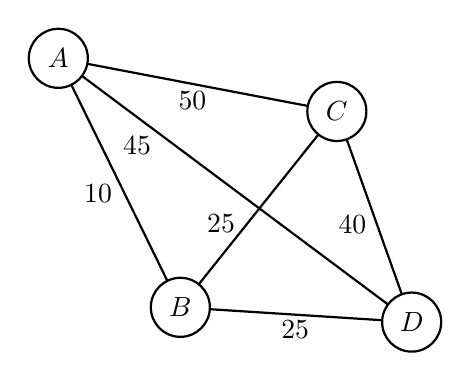
\begin{tikzpicture}[scale=0.125]
                \tikzstyle{every node}+=[inner sep=0pt]
                \draw  [thick](22,-14.2) circle (3);
                \draw  [][thick](22,-14.2) node {$A$};
                \draw  [thick](34.4,-39.5) circle (3);
                \draw  [][thick](34.4,-39.5) node {$B$};
                \draw  [thick](50.3,-19.6) circle (3);
                \draw  [][thick](50.3,-19.6) node {$C$};
                \draw  [thick](57.9,-41) circle (3);
                \draw  [][thick](57.9,-41) node {$D$};
                \draw  [][thick](23.32,-16.89) -- (33.08,-36.81);
                
                \draw [](27.5,-27.94) node [left] {$10$};
                \draw [][thick] (24.95,-14.76) -- (47.35,-19.04);
                
                \draw [](35.62,-17.49) node [below] {$50$};
                \draw [][thick] (51.3,-22.43) -- (56.9,-38.17);
                
                \draw [](53.34,-31.06) node [left] {$40$};
                \draw [][thick] (37.39,-39.69) -- (54.91,-40.81);
                
                \draw [](46.07,-40.81) node [below] {$25$};
                \draw [][thick] (24.4,-15.99) -- (55.5,-39.21);
                
                \draw [](30,-24) node [above] {$45$};
                \draw [][thick] (48.43,-21.94) -- (36.27,-37.16);
                
                \draw [](40, -31) node [left] {$25$};
            \end{tikzpicture}
        \end{center}
        \caption{\doublespacing An example of a TSP Instance}
        \label{fig:lattice}
    \end{figure}

    \subsubsection{Creating a Better Lower Bound}
    Firstly, our lower bound calculation before our heuristic is simply the sum 
    of the tour edges. To improve this we will utilize an encoding scheme known as 
    a graph adjacency matrix, and reduce it. There are two reasons for the reduction, 
    the first is that reduction keeps track of our current state of the tour, and the second
    is that the cost of reduction is an admissible heuristic in the TSP problem.
    The idea is that the cost of reduction is equal to the shortest possible edges left to
    take on the graph. Note, the shortest edges do not have to be constrained to the tour, they
    are just simply the shortest edges coming out of each node. To compute the reduction, take the
    shortest number in each row, then subtract it from each element, finally sum the shortest edges.
    The output matrix becomes the new state of the child branch and used to compute it's lower-bound.\\
    
    \begin{figure}
        \begin{minipage}{.5\linewidth}
          \centering
          \begin{equation*}
            A = 
            \begin{vmatrix}
                \infty & 10 & 50 & 45\\
                10 & \infty & 25 & 25 \\
                50 & 25 & \infty & 40 \\
                45 & 25 & 40 & \infty
	        \end{vmatrix}
          \end{equation*}
          Matrix for TSP instance in Figure 5.
        \end{minipage}%
        \begin{minipage}{.5\linewidth}
          \centering
          \begin{equation*}
	        %!c = 2 + 3 + 2 + 3
            A^{'} = 
                \begin{vmatrix}
                    \infty & 0 & 40 & 35\\
                    0 & \infty & 15 & 15 \\
                    25 & 0 & \infty & 15 \\
                    20 & 0 & 15 & \infty
                \end{vmatrix}
            \end{equation*}
          Row reduced matrix of matrix $A$\\
        \end{minipage}
        \caption{First reduction matrix of TSP instance in Figure 5.
                The cost of reduction $ R(A) = 10 + 10 + 25 + 25 = 70$}
      \end{figure}
      

    After computing the reduction cost we can now make our lower bound calculation.
    \begin{equation}
        LB = LB_p + w(p, n) + R(M_n)
    \end{equation}
    Where $LB_p$ is the lower-bound of the parent, $w(p, n)$ is the weight of the edge
    between the parent, and $R(M_n)$ is the cost of reduction.\\

    \subsubsection{Preformance Gain}
    It is important to realize that branch and bound is not one size fits all algorithm, so
    although there may be a problem that can be encoded with an adjacency matrix, it does not mean
    there exists an admissible heuristic for it. Creating a better lower bound by using a heuristic
    can provide performance gains, but again it is problem dependent.


    \begin{figure}
        \begin{minipage}{.5\linewidth}
          \centering
          \begin{center}
            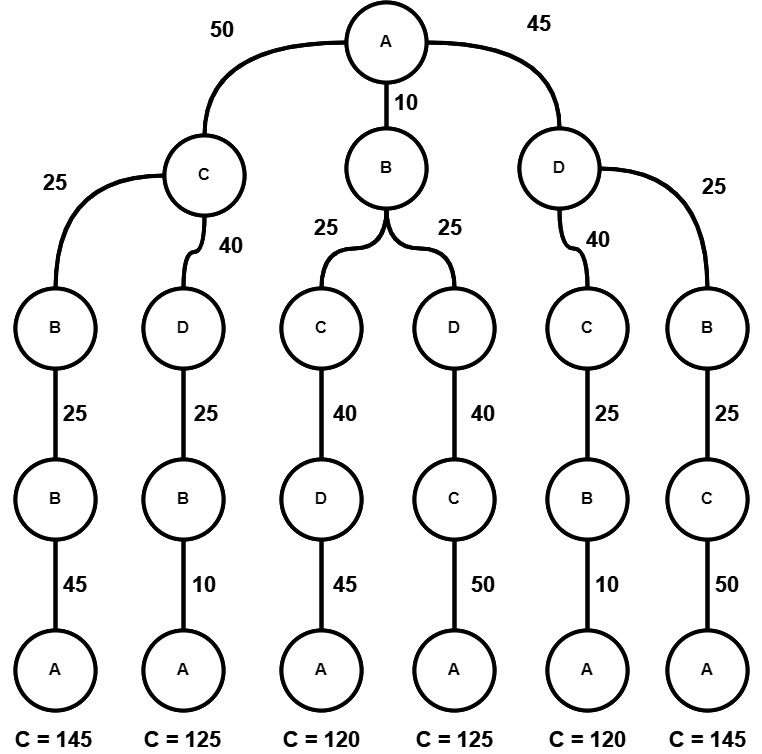
\includegraphics[width=6cm]{images/BnB-TSP-1.jpg}
        \end{center}
        \captionsetup{labelformat=empty}
        \caption{\doublespacing Tree generated without heuristic.}
        \end{minipage}%
        \begin{minipage}{.5\linewidth}
            \centering
            \begin{center}
              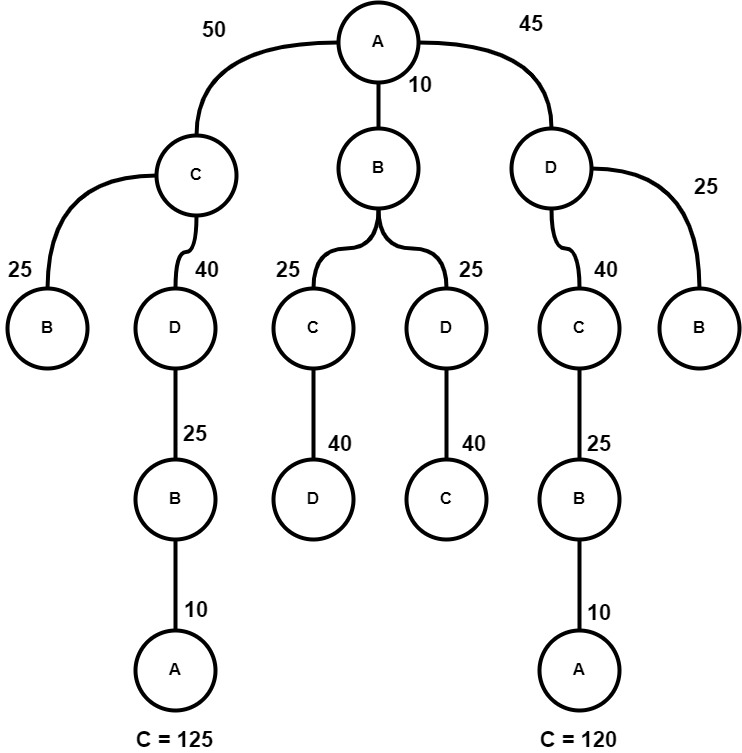
\includegraphics[width=6cm]{images/BnB-TSP-2.jpg}
          \end{center}
          \captionsetup{labelformat=empty}
          \caption{\doublespacing Tree generated with row reduction heuristic.}
          \end{minipage}
        \caption{\doublespacing An example of 
        the trees generated with and without a heuristic for the TSP instance in Figure 5.}
    \end{figure}

   

	
	%! Author = rickr
%! Date = 11/17/2021

\section{Advancing Branch And Bound}

	
	%! Author = rickr
%! Date = 11/17/2021
\newpage
\section{Traveling Salesman Problem To Ising Model}
	Recent interest in solving NP-complete and NP-hard problems via adiabatic quantum optimization has led to convenient transformations of Ising formulations. 
	The idea is that if one problem has a quantum Hamiltonian $H_p$ whose ground state energy encodes the solution to a problem of interest, and another Hamiltonian $H_0$, whose ground state is "easy" to find and prepare, then we can prepare the system to be in the ground state of $H_0$ before adiabatically changing it in terms of $H_p$ for a time $T$ \cite{lucas2014ising}. 
	So long as $T$ is large enough and $H_0$ and $H_p$ do not commute, the system should remain in the resulting ground state for all time. 
	Therefore, measuring the ground state of the system at time $T$ will return a solution to the problem of interest. 
	Though there has been debate on the practicality of such a method, there has been extensive effort in finding formulations of various NPC and NPH problems in terms of Ising models. 
	Here we present one such transformation and show how it can be used to improve the computation time of a generic Branch-and-Bound technique. 
	
	%! Author = rickr
%! Date = 11/27/2021
\subsection{TSP to Hamiltonian Circuit}
Consider an instance of the Traveling Salesman problem for the graph $G = (V,E)$ as shown in Figure \ref{fig:tsp}.
Each edge $uv$ has a weight $W_{uv}$ associated with it. 
\begin{figure}[h]
	\begin{center}
		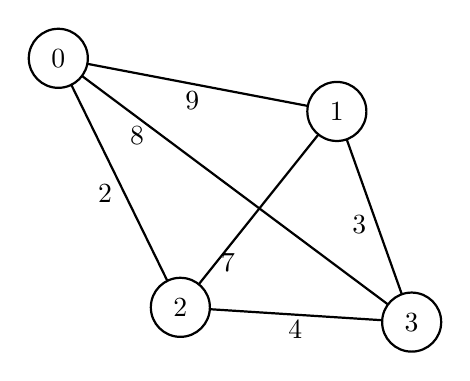
\begin{tikzpicture}[scale=0.125]
			\tikzstyle{every node}+=[inner sep=0pt]
			\draw  [thick](22,-14.2) circle (3);
			\draw  [][thick](22,-14.2) node {$0$};
			\draw  [thick](34.4,-39.5) circle (3);
			\draw  [][thick](34.4,-39.5) node {$2$};
			\draw  [thick](50.3,-19.6) circle (3);
			\draw  [][thick](50.3,-19.6) node {$1$};
			\draw  [thick](57.9,-41) circle (3);
			\draw  [][thick](57.9,-41) node {$3$};
			\draw  [][thick](23.32,-16.89) -- (33.08,-36.81);
			
			\draw [](27.5,-27.94) node [left] {$2$};
			\draw [][thick] (24.95,-14.76) -- (47.35,-19.04);
			
			\draw [](35.62,-17.49) node [below] {$9$};
			\draw [][thick] (51.3,-22.43) -- (56.9,-38.17);
			
			\draw [](53.34,-31.06) node [left] {$3$};
			\draw [][thick] (37.39,-39.69) -- (54.91,-40.81);
			
			\draw [](46.07,-40.81) node [below] {$4$};
			\draw [][thick] (24.4,-15.99) -- (55.5,-39.21);
			
			\draw [](30,-23) node [above] {$8$};
			\draw [][thick] (48.43,-21.94) -- (36.27,-37.16);
			
			\draw [](40, -35) node [left] {$7$};
		\end{tikzpicture}
		\caption{\doublespacing A graph G representing an instance of the Traveling Salesman Problem. Each node $V$ is connected via a weighted edge $E=W_{uv}$.}
		\label{fig:tsp}
	\end{center}
\end{figure}
The set of solutions to this graph can be seen in Table \ref{tab:eigenset} located in the appendix and the shortest Hamiltonian cycle that can be taken has a total distance of 18.
One possible route is $2\rightarrow3\rightarrow1\rightarrow0$. 
This route can be represented as a matrix as shown if Figure \ref{fig:matrix}, where $i$ and $p$ correspond to the city and order of traversal respectively. 
\begin{figure}[h]
	\begin{center}
		\begin{tabular}{c|cccc}
			\backslashbox{i}{p}&0 &1 &2 &3 \\
			\hline
			0& 0&0&0&1\\
			
			1& 0&0&1&0\\
			
			2& 1&0&0&0\\
			
			3& 0&1&0&0\\
		\end{tabular}
	\end{center}\caption{\doublespacing Solution to TSP in Figure \ref{fig:tsp} represented in the form of a matrix. The column $i$ represents each node, and the row $p$ corresponds to the nodes position in the traversal. A decision variable value of 1 corresponds to the path being taken.}\label{fig:matrix}
\end{figure}
The solution matrix of Figure \ref{fig:matrix} can be unpacked into the form of a vector 
\begin{equation}
	\vec{x} = \langle x_1, x_2, \dots, x_{N^2} \rangle
	\label{eq:vector}
\end{equation}
such that $x_j = x_{N \cdot i+p}$ where $N$ is the number of nodes in the graph. 
For example, the value at $x_{2,1}$ in the matrix will map to $x_9$ in the vector. Therefore, the vector representation of the solution to TSP in Figure \ref{fig:tsp} is $\vec{x} = <0,0,0,1,0,0,1,0,1,0,0,0,0,1,0,0>$. 
Applying the cost function to the eigenvector will result in an eigenvalue (the total distance traveled) of $C(\vec{x}) = 18$.

For nodes forming a traversal such that $x_{i,p}$ and $x_{i,p+1}$ are both equal to one but not connected in $G$, i.e., $(i,j)\notin E$, then an energy penalty should be imposed in the form $\sum_{i,j \notin E}\sum_p x_{i,p}x_{i,p+1}>0$ \cite{lucas2014ising}.
However, since we are only considering fully connected graphs, this term may be omitted and the net cost of a tour can be calculated from the cost function of Equation \ref{eq:cost}.
% Cost Function
\begin{equation}
	C(X)=\sum_{i,j}w_{i,j} \sum_p x_{i,p}x_{j,p+1} 
	\label{eq:cost}
\end{equation}
Where $w_{i,j}$ is the weight between nodes $i$ and $j$, and $x_{i,p}x_{j,p+1}=1$ if the route is actually taken. Inspecting the features of Figure \ref{fig:matrix}, we find that every vertex can only appear once in a cycle and each position must be occupied by a node. 
This amounts to the two constraints given in Equation \ref{eq:constraints}.
% Constraints
\begin{equation}
	\sum_p x_{i,p}=1 \quad \forall \: i \in cities \quad \text{and} \quad \sum_i x_{i,p}=1 \quad \forall \: p \in route
	\label{eq:constraints}
\end{equation}

By imposing these constraints to Equation \ref{eq:cost}, we find that the objective function to be minimized takes the form
% Distance with constraints
\begin{equation}
	C(X)=\sum_{i,j}w_{i,j} \sum_p x_{i,p}x_{j,p+1} + A\sum_p (1 - \sum_i x_{i,p})^2 + A\sum_i (1 - \sum_p x_{i,p})^2
	\label{eq:hamiltoniancircuit}
\end{equation}
where $A>W_{max}$ is a positive constant set to be much larger than maximum weight encountered during the traversal. Note that the constraints are squared so as to prevent the algorithm from diverging to negative infinity. 

To complete the preparation of TSP, we need to convert the cost function of Equation \ref{eq:cost} into a quantum Hamiltonian by changing variables from $x_i$ to the Pauli operator $\sigma_i^z$ (a $2x2$ matrix whose eigenvectors $|1,0\rangle$ and $|0,-1\rangle$ have eigenvalues (+1,-1)). 
\begin{equation}
	x_i \rightarrow \frac{ 1-\sigma_{i,p}^z}{2} \qquad \Rightarrow \qquad C(X) \rightarrow C(\sigma_{i,p}^z) \equiv H_p
	\label{eq:transformation}
\end{equation}
	%! Author = rickr
%! Date = 11/27/2021
\subsection{The Ising Model}
In ideal \textit{paramagnetism} (magnetism where materials are weakly attracted by an external magnetic field) microscopic magnetic dipole moments respond only to an external field. 
However, in the real world, neighboring atomic dipoles are influenced by each other. 
When neighboring dipoles align parallel, even in the absence of an external field, we call the material a ferromagnet. 
The Ising model is a mathematical model used to describe ferromagnetism in terms of statistical mechanics. The model consists of discrete variables that represent the magnetic dipole moments of atomic spins and can have a value of $\pm 1$. 
The variables are used to describe preference for neighboring dipoles to align parallel or anti-parallel to each other \cite{schroeder2011thermal}.
\begin{figure}[h]
	\begin{center}
		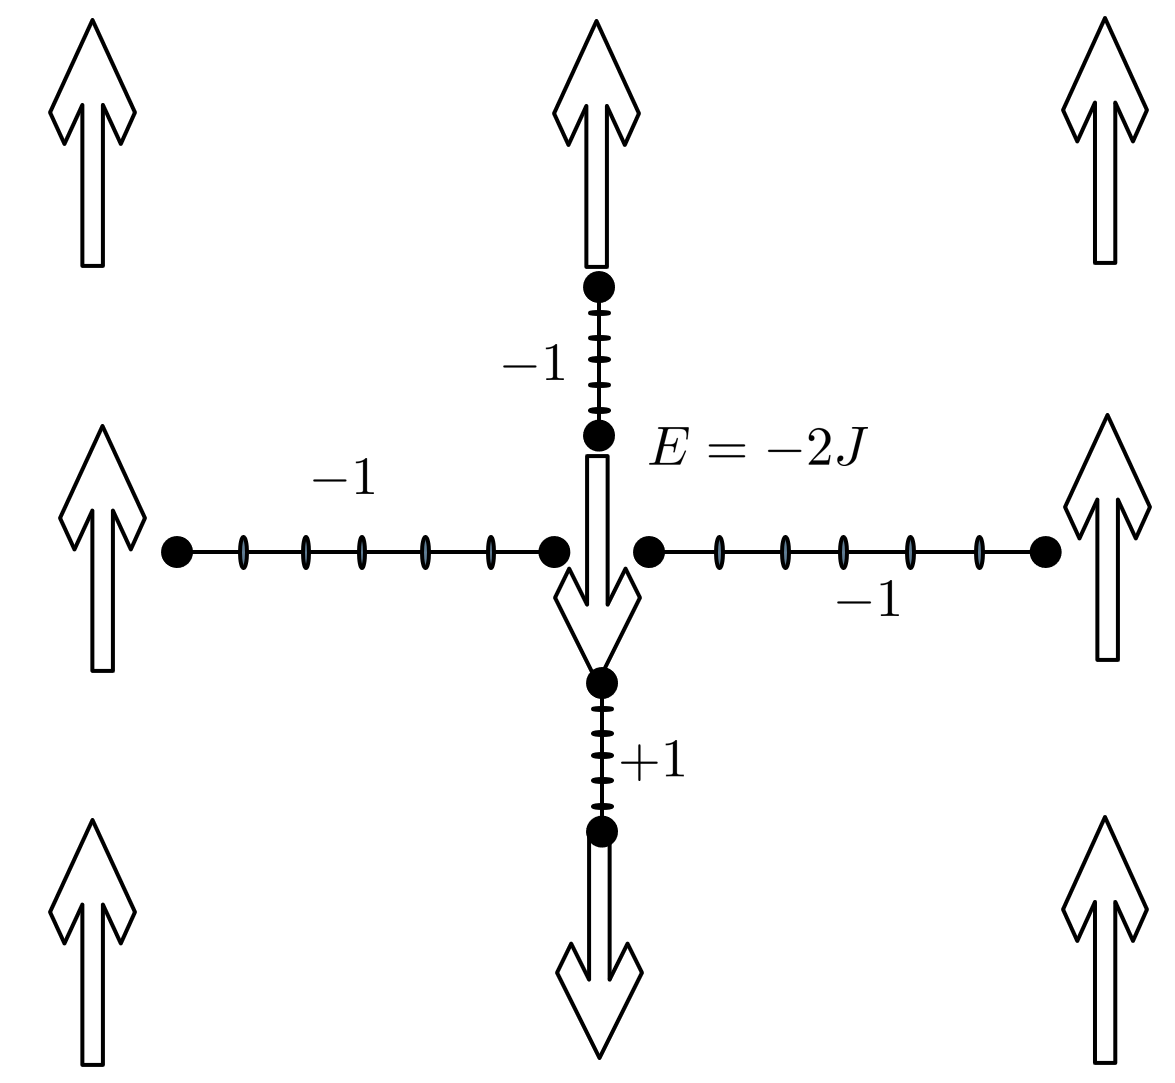
\includegraphics[width=6cm]{images/lattice}
	\end{center}
	\caption{\doublespacing Atomic spin states arranged into a 2-dimensional lattice structure under periodic boundary conditions. The energy of the particle at lattice site $k$ has a value $E = -2J$ and the total energy of the system is found by summing over the entire structure.}
	\label{fig:lattice}
\end{figure}

For example, consider a lattice of particles as shown in Figure \ref{fig:lattice}. 
Each particle has an associated spin state that can take the orientations of spin-up $|+\rangle$ or spin-down $|-\rangle$ with values $\sigma_k = +1$ and $\sigma_k = -1$ respectively. The energy associated with the particle at lattice site $k$ is found to be 
\begin{equation}
	E_k= - J\sum_{<i,j>}\sigma_k^i\sigma_k^j \quad \cite{ising1925beitrag}
	\label{eq:latticeSiteEnergy}
\end{equation}
where $J$ is a coupling constant, $\sigma_k$ is a discrete variable, and $<i,j>$ means to sum over the nearest neighbors. Note that for parallel spins, $J>0$, for anti-parallel spins $J<0$, and for no interaction $J = 0$. 
In the presence of a magnetic field $\vec{B}$, the kinetic and potential energy of the system can be represented by the Hamiltonian
\begin{equation}
	H_0 = \frac{g_s}{2}\mu_B B\sum_{i=1}^N \sigma_z^i - J\sum_{<i,j>}\sigma_z^i\sigma_z^j
	\label{eq:isingHamiltonian}
\end{equation} 
where the spin g-factor for an electron $g_s$ and the Bohr magneton $\mu_B$ are constants, and the discrete variable $\sigma_k$ has been replaced with the Pauli z-operator $\sigma_z$ as in Equation \ref{eq:transformation}. 
There are many techniques for solving generalized Ising models including transfer matrix methods\cite{onsager1944crystal}, graphical/combinatorial methods\cite{feynman1972statistical}, and Monte Carlo simulations\cite{schroeder2011thermal}. 
However, with the advent of quantum computation, the time independent Schrodinger equation is especially convenient.
	%! Author = rickr
%! Date = 11/27/2021
\subsection{Time Independent Schrodinger Equation}
In quantum mechanics, the Schrodinger equation is a partial differential equation that governs the dynamics of the wave function $\Psi(x,t)$ of a particle in a system. 
In essence, it is an accounting of energy where the kinetic and potential energy are encapsulated in a single operator called a Hamiltonian, and the total energy of the system is set to be the time derivative acting on the wave function. 
Since the Ising model focuses on the spin configuration of a particle and neglects the space and time components, we can utilize a time independent version of the Schrodinger equation and treat it as an eigenvalue problem as shown in Equation \ref{eq:tise}. 

\begin{equation}
	H | \Psi \rangle = E | \Psi \rangle
	\label{eq:tise}
\end{equation}

As the Hamiltonian operator acts on the wave function, a scalar value is produced along with the same vector. 
In terms of linear algebra, the wave function $| \Psi \rangle$ can be treated as an eigenvector with a corresponding eigenvalue $E$. 
Note that each eigenvalue can correspond to a set of eigenvectors and that minimizing Equation \ref{eq:tise} is to solve for the ground state energy of the system. \\

Relating this back to the Traveling Salesman problem, recall that in Equation \ref{eq:transformation} we transformed the cost function into the same form as the Ising Hamiltonial of Equation \ref{eq:isingHamiltonian}. We now need to map the solution vector of Equation \ref{eq:vector} into qubits to be fed into a quantum computer. 
\begin{equation}
	\vec{x} = \langle x_1, x_2, \dots, x_{N^2} \rangle \rightarrow |\Psi\rangle = |x_1\rangle \otimes |x_2\rangle \dots \otimes  |x_{N^2}\rangle 
\end{equation}
Note that we do not require a transformation between the energy of the Schrodinger equation and the distance of the Hamiltonian Circuit because both quantities are scalars. This completes the transformation from the Traveling Salesman problem into the Ising model. The solution for the ground state energy of the Ising Hamiltonian corresponds directly to the minimum tour distance in TSP, however, in this form we are able to exploit the features of quantum mechanics and obtain a solution in far less time. 
	

	
	%! Author = rickr
%! Date = 11/17/2021
\section{Quantum Improvements}
	With the recent advancements in quantum computing, access to hardware has become readily available to the general public and quantum algorithms have been shown to perform exponentially better than some of their classical counterparts for select problems. 
	For example, Grover's algorithm can sort through and find an element within an unstructured set using $O(\sqrt{N})$ operations as oppose to the $O(N)$ performance of an exhaustive search. However, for many problems, it's is more beneficial to utilize techniques found in classical algorithms that take advantage of the structure of a problem. One such technique is Branch-and-bound. 
	By applying the Branch-and-Bound paradigm in a quantum setting, it is possible to achieve a near quadratic improvement beyond that of classical pruning techniques \cite{montanaro2020quantum}. 

	Though there are several different implementations of quantum computing systems, the most popular is the quantum circuit.
	The model is based on the concept of a qubit which is analogous to the bit in classical computing. 
	The qubit acts as the basic unit of quantum information and is physically realized as the spin state of a fermion (a particle with a half integer spin; typically 1/2). 
	Since the qubit is measured as the spin state of a particle, it's properties are governed by the wave function of that particle $|\Psi\rangle$. 
	For example, since the quantum spin number of a qubit is 1/2, it can exist in one of two states (spin up $|0\rangle$ or spin down $|1\rangle$) when measured. 
	However, before the measurement, the particle can be in a superposition of both states 
	\begin{equation}
		|\Psi\rangle = \alpha |0\rangle + \beta|1\rangle
		\label{eq:spinStates}
	\end{equation}
	where $\alpha$ and $\beta$ are probability amplitudes such that $|\alpha|^2+|\beta|^2 = 1$.
	It is only when the wave-function is measured that it actually collapse in a definite value of $|0 \rangle$ or $|1\rangle$.
	This means that unlike a classical bit that can discretely take on a value of $0$ \textit{or} $1$, the qubit can exist in a state of $0$ \textit{and} $1$ simultaneously. We can exploit this feature of quantum mechanics to increase the speed of classical algorithms by placing the qubit into a superposition of states and letting the system evolve in time before taking a measurement. 
	
	%! Author = rickr
%! Date = 11/27/2021
\subsection{Classical vs Quantum Walk}

Consider the case of a classical random walk. In this example we search for a marked node within a binary tree of size $n$ nodes. 
If we have no indication of where in the tree the target might be, then a sure proof way of finding it is to visit each node, one step at a time, with $50\%$ probability of taking a step to the left and $50\%$ probability of taking a step to the right. 
Naturally, for every step away from the origin, there is an equal probability of taking a step back toward the origin, and over time we will obtain a normal Gaussian distribution of steps as shown in Figure \ref{fig:quantumWalk}. 
The classical random walk distribution exhibits a variance of 
\begin{equation}
	\sigma^2 \propto n
\end{equation}
which is to say that there is a very low probability of hitting the target if it is far away from the origin.
Since  each step is based on a set of definite states, the randomness of the traversal is caused by a stochastic transition between states.
Now consider a random walk in a quantum setting. 
In this case, the randomness comes from the quantum superposition imposed by Equation \ref{eq:spinStates}, a reversible unitary evolution (typically in the form of a Hadamard coin), and a collapse of the wave-function when a measurement is actually taken. 
Another difference between the quantum and classical random walk is the time at which a measurement is taken. 
In the classical version, it makes no difference to take measurements at each iteration, however in the quantum version, if a measurement of the wave-function is taken at each iteration, then the distribution converges to the classical Gaussian form. 
If the wave-function is left to interfere with itself before a measurement is taken, then the probability distribution is much more intricate, as can be seen in Figure \ref{fig:quantumWalk}.
It can be shown the after $n$ steps, the quantum walk obtains a variance of 
\begin{equation}
	\sigma^2 \propto n^2 \quad\cite{kempe2003quantum}
\end{equation}
Therefore, the quantum walk propagates quadratically faster than the classical walk, and this speed increase can be applied to the branch-and-bound framework. 
From Figure \ref{fig:quantumWalk}, if the wave-function is placed in a superposition, then the distribution exhibits destructive interference about the origin.
However, if the wave-function begins in a pure spin-up or spin-down configuration, then it is possible to create a bias toward any particular direction as shown in Figure \ref{fig:biasWalk} of the appendix.
\begin{figure}[H]
	\begin{center}
		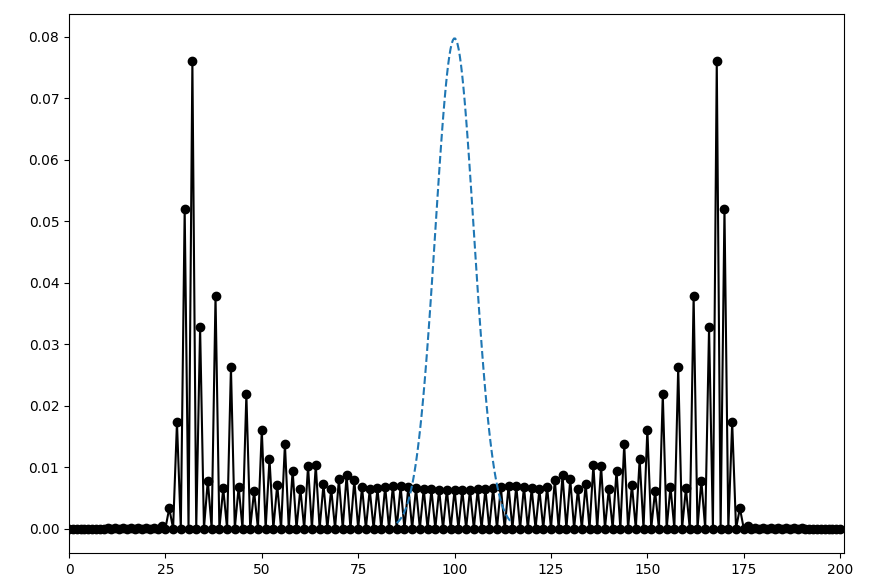
\includegraphics[width=12cm]{images/afunc2}
	\end{center}
	\caption{\doublespacing Difference between quantum and classical random walk. The blue dotted line represents the Gaussian distribution created by the classical walk and has a variance $\sigma^2 \propto n$. The black distribution is the result of the quantum random walk where the initial wave-function placed into a superposition $|\Psi\rangle = \alpha|0\rangle + \beta|1\rangle$ and acted on my a balanced Hadamard coin. The quantum distribution exhibits a variance of $\sigma^2 \propto n$ with de-constructive interference about the origin and constructive interference at the edges of propagation.}
	\label{fig:quantumWalk}
\end{figure}
\noindent
To summarize the results, consider three individual cases of solving combinatorial problems with Hamiltonians similar to that of Equation \ref{eq:isingHamiltonian}.
One case is solved using classical branch-and-bound techniques, one is solved using quantum walks, and one is solved using branch-and-bound in a quantum setting. 
If the classical branch-and-bound techniques are applied to solve for the largest known ground states of the Beransconi model, the runtime is roughly $O(2^{0.79n})$ \cite{packebusch2016low}. 
If we apply a quantum walk to classical algorithms that solve the Sherrington-Kirkpatrick model (an Ising model with long range anti-ferrmagnetic couplings) then it has been shown we can increase runtime to approximately $O(2^{0.41n})$ \cite{callison2019finding}. 
Finally, by applying quantum branch-and-bound algorithms to the same model, it has been shown that the runtime can be increased further to $O(2^{0.226n})$ \cite{montanaro2020quantum}.

	
	\input{sections/Conclusion.tex}
	
	\bibliographystyle{IEEEtran}
	\bibliography{groupPaper}
	
	\newpage\appendix
	\begin{table}[h]
		\[
		\begin{split}
			&0 \rightarrow 1 \rightarrow 2 \rightarrow 3 \rightarrow 0 \quad \text{dist}=28 \hspace{1cm} 1 \rightarrow 0 \rightarrow 2 \rightarrow 3 \rightarrow 1 \quad \text{dist}=18 \\
			&0 \rightarrow 1 \rightarrow 3 \rightarrow 2 \rightarrow 0 \quad \text{dist}=18 \hspace{1cm} 1 \rightarrow 0 \rightarrow 3 \rightarrow 2 \rightarrow 1 \quad \text{dist}=28\\
			&0 \rightarrow 2 \rightarrow 1 \rightarrow 3 \rightarrow 0 \quad \text{dist}=20 \hspace{1cm} 1 \rightarrow 2 \rightarrow 0 \rightarrow 3 \rightarrow 1 \quad \text{dist}=20\\
			&0 \rightarrow 2 \rightarrow 3 \rightarrow 1 \rightarrow 0 \quad \text{dist}=18 \hspace{1cm} 1 \rightarrow 2 \rightarrow 3 \rightarrow 0 \rightarrow 1 \quad \text{dist}=28\\
			&0 \rightarrow 3 \rightarrow 1 \rightarrow 2 \rightarrow 0 \quad \text{dist}=20 \hspace{1cm} 1 \rightarrow 3 \rightarrow 0 \rightarrow 2 \rightarrow 1 \quad \text{dist}=20\\
			&0 \rightarrow 3 \rightarrow 2 \rightarrow 1 \rightarrow 0 \quad \text{dist}=28 \hspace{1cm} 1 \rightarrow 3 \rightarrow 2 \rightarrow 0 \rightarrow 1 \quad \text{dist}=18\\ 
			&2 \rightarrow 0 \rightarrow 1 \rightarrow 3 \rightarrow 2 \quad \text{dist}=18 \hspace{1cm} 3 \rightarrow 0 \rightarrow 1 \rightarrow 2 \rightarrow 3 \quad \text{dist}=28 \\
			&2 \rightarrow 0 \rightarrow 3 \rightarrow 1 \rightarrow 2 \quad \text{dist}=20 \hspace{1cm} 3 \rightarrow 0 \rightarrow 2 \rightarrow 1 \rightarrow 3 \quad \text{dist}=20\\
			&2 \rightarrow 1 \rightarrow 0 \rightarrow 3 \rightarrow 2 \quad \text{dist}=28 \hspace{1cm} 3 \rightarrow 1 \rightarrow 0 \rightarrow 2 \rightarrow 3 \quad \text{dist}=18\\
			&2 \rightarrow 1 \rightarrow 3 \rightarrow 0 \rightarrow 2 \quad \text{dist}=20 \hspace{1cm} 3 \rightarrow 1 \rightarrow 2 \rightarrow 0 \rightarrow 3 \quad \text{dist}=20\\
			&2 \rightarrow 3 \rightarrow 0 \rightarrow 1 \rightarrow 2 \quad \text{dist}=28 \hspace{1cm} 3 \rightarrow 2 \rightarrow 0 \rightarrow 1 \rightarrow 3 \quad \text{dist}=18\\
			&2 \rightarrow 3 \rightarrow 1 \rightarrow 0 \rightarrow 2 \quad \text{dist}=18 \hspace{1cm} 3 \rightarrow 2 \rightarrow 1 \rightarrow 0 \rightarrow 3 \quad \text{dist}=28\\
		\end{split}
		\]
		\caption{\doublespacing Solutions to TSP in Figure \ref{fig:tsp}. 
			Each eigenvector forms a tour about the graph with an associated eigenvalue corresponding to the total distance traveled. 
			The optimal ground state eigenvalue 18 corresponds to a set of possible eigenvectors.}
		\label{tab:eigenset}
	\end{table}
\vspace{-0.5cm}
		\begin{figure}[H]
				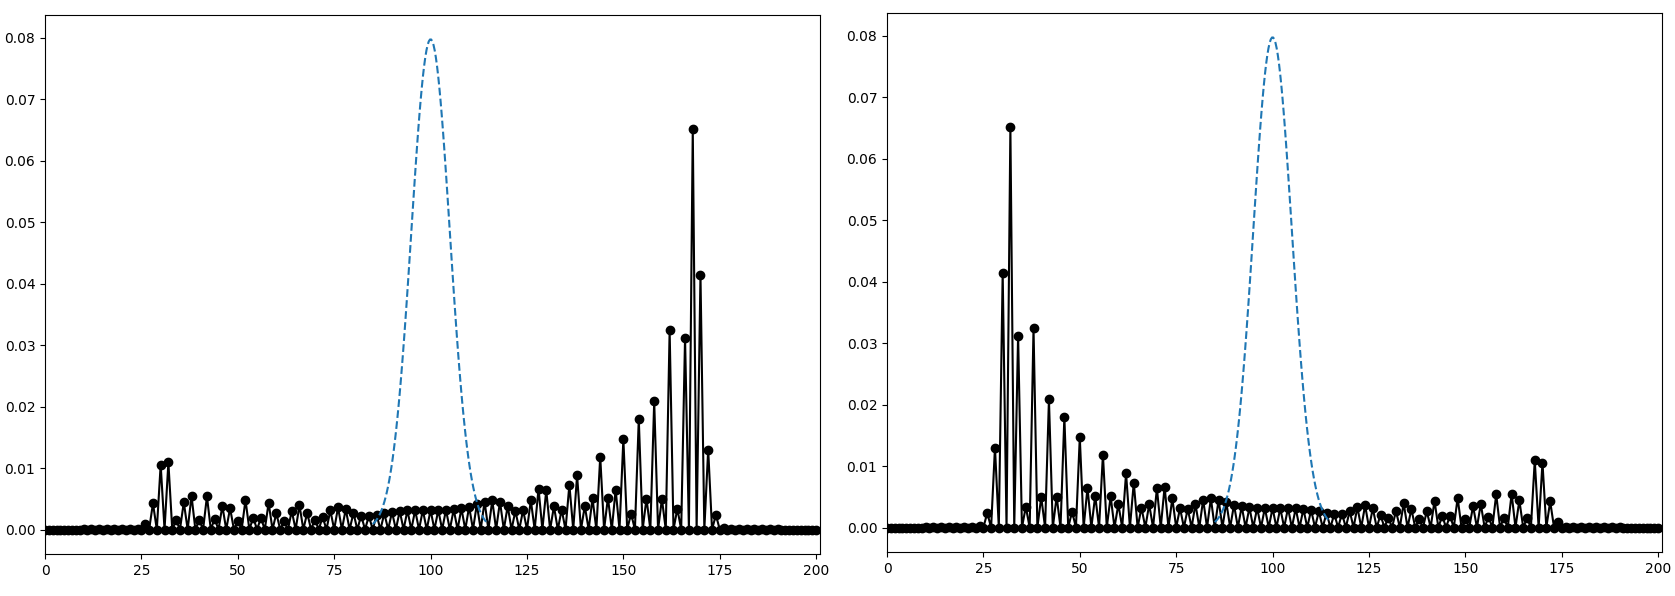
\includegraphics[width=16cm]{images/bias}
			\caption{\doublespacing Plot of the probability distributions of a classical random walk and a quantum random walk. 
				The blue dotted line in each plot is the result of a classical Gaussian distribution. 
				In the left plot, the black distribution is the result of preparing the quantum walk with a particle in a pure spin-up configuration $|\Psi\rangle = |0\rangle$. 
				In the right plot, the particle is prepared in a spin-down configuration $|\Psi\rangle = |1\rangle$. 
				In both cases, the quantum distribution exhibits de-constructive interference about the origin, however it is possible to impose a bias toward a particular direction simply by initializing the system with different weights in $\alpha$ and $\beta$ from Equation \ref{eq:spinStates}.}
			\label{fig:biasWalk}
		\end{figure}

	
	
\end{document}